\IfFileExists{acmart.cls}{%
  \documentclass[sigconf,nonacm]{acmart}
  \newif\ifusingacmart
  \usingacmarttrue
}{%
  \documentclass[11pt]{article}
  \newif\ifusingacmart
  \usingacmartfalse
}

\ifusingacmart
  \settopmatter{printacmref=false}
  \renewcommand\footnotetextcopyrightpermission[1]{}
  \setcopyright{none}
  \acmConference[DSC 148 Project]{DSC 148: Introduction to Data Mining}{Spring 2026}{University of California, San Diego}
  \acmYear{2026}
  \copyrightyear{2026}
  \acmDOI{}
  \acmISBN{}
\else
  \usepackage[margin=0.72in]{geometry}
\fi

\AtBeginDocument{%
  \providecommand\BibTeX{{Bib\TeX}}}

\usepackage{amsmath}
\usepackage{amssymb}
\usepackage{booktabs}
\usepackage{graphicx}
\usepackage{subcaption}
\usepackage{caption}
\usepackage{float}
\IfFileExists{placeins.sty}{\usepackage{placeins}}{\newcommand{\FloatBarrier}{\relax}}
\usepackage{array}
\usepackage{tabularx}
\usepackage{url}
\ifusingacmart
\else
  \usepackage[hidelinks]{hyperref}
\fi
\PassOptionsToPackage{hyphens}{url}
\urlstyle{same}
\providecommand{\Description}[1]{}
\providecommand{\keywords}[1]{\par\smallskip\noindent\textbf{Keywords:} #1\par}
\captionsetup{font=small, skip=4pt}
\setlength{\textfloatsep}{8pt plus 2pt minus 2pt}
\setlength{\floatsep}{8pt plus 2pt minus 2pt}
\setlength{\intextsep}{8pt plus 2pt minus 2pt}
\setcounter{topnumber}{3}
\setcounter{bottomnumber}{2}
\setcounter{totalnumber}{5}
\renewcommand{\topfraction}{0.9}
\renewcommand{\bottomfraction}{0.8}
\renewcommand{\textfraction}{0.08}
\renewcommand{\floatpagefraction}{0.85}
\emergencystretch=1.5em
\raggedbottom

\newcommand{\headervisual}{%
  \begin{center}
    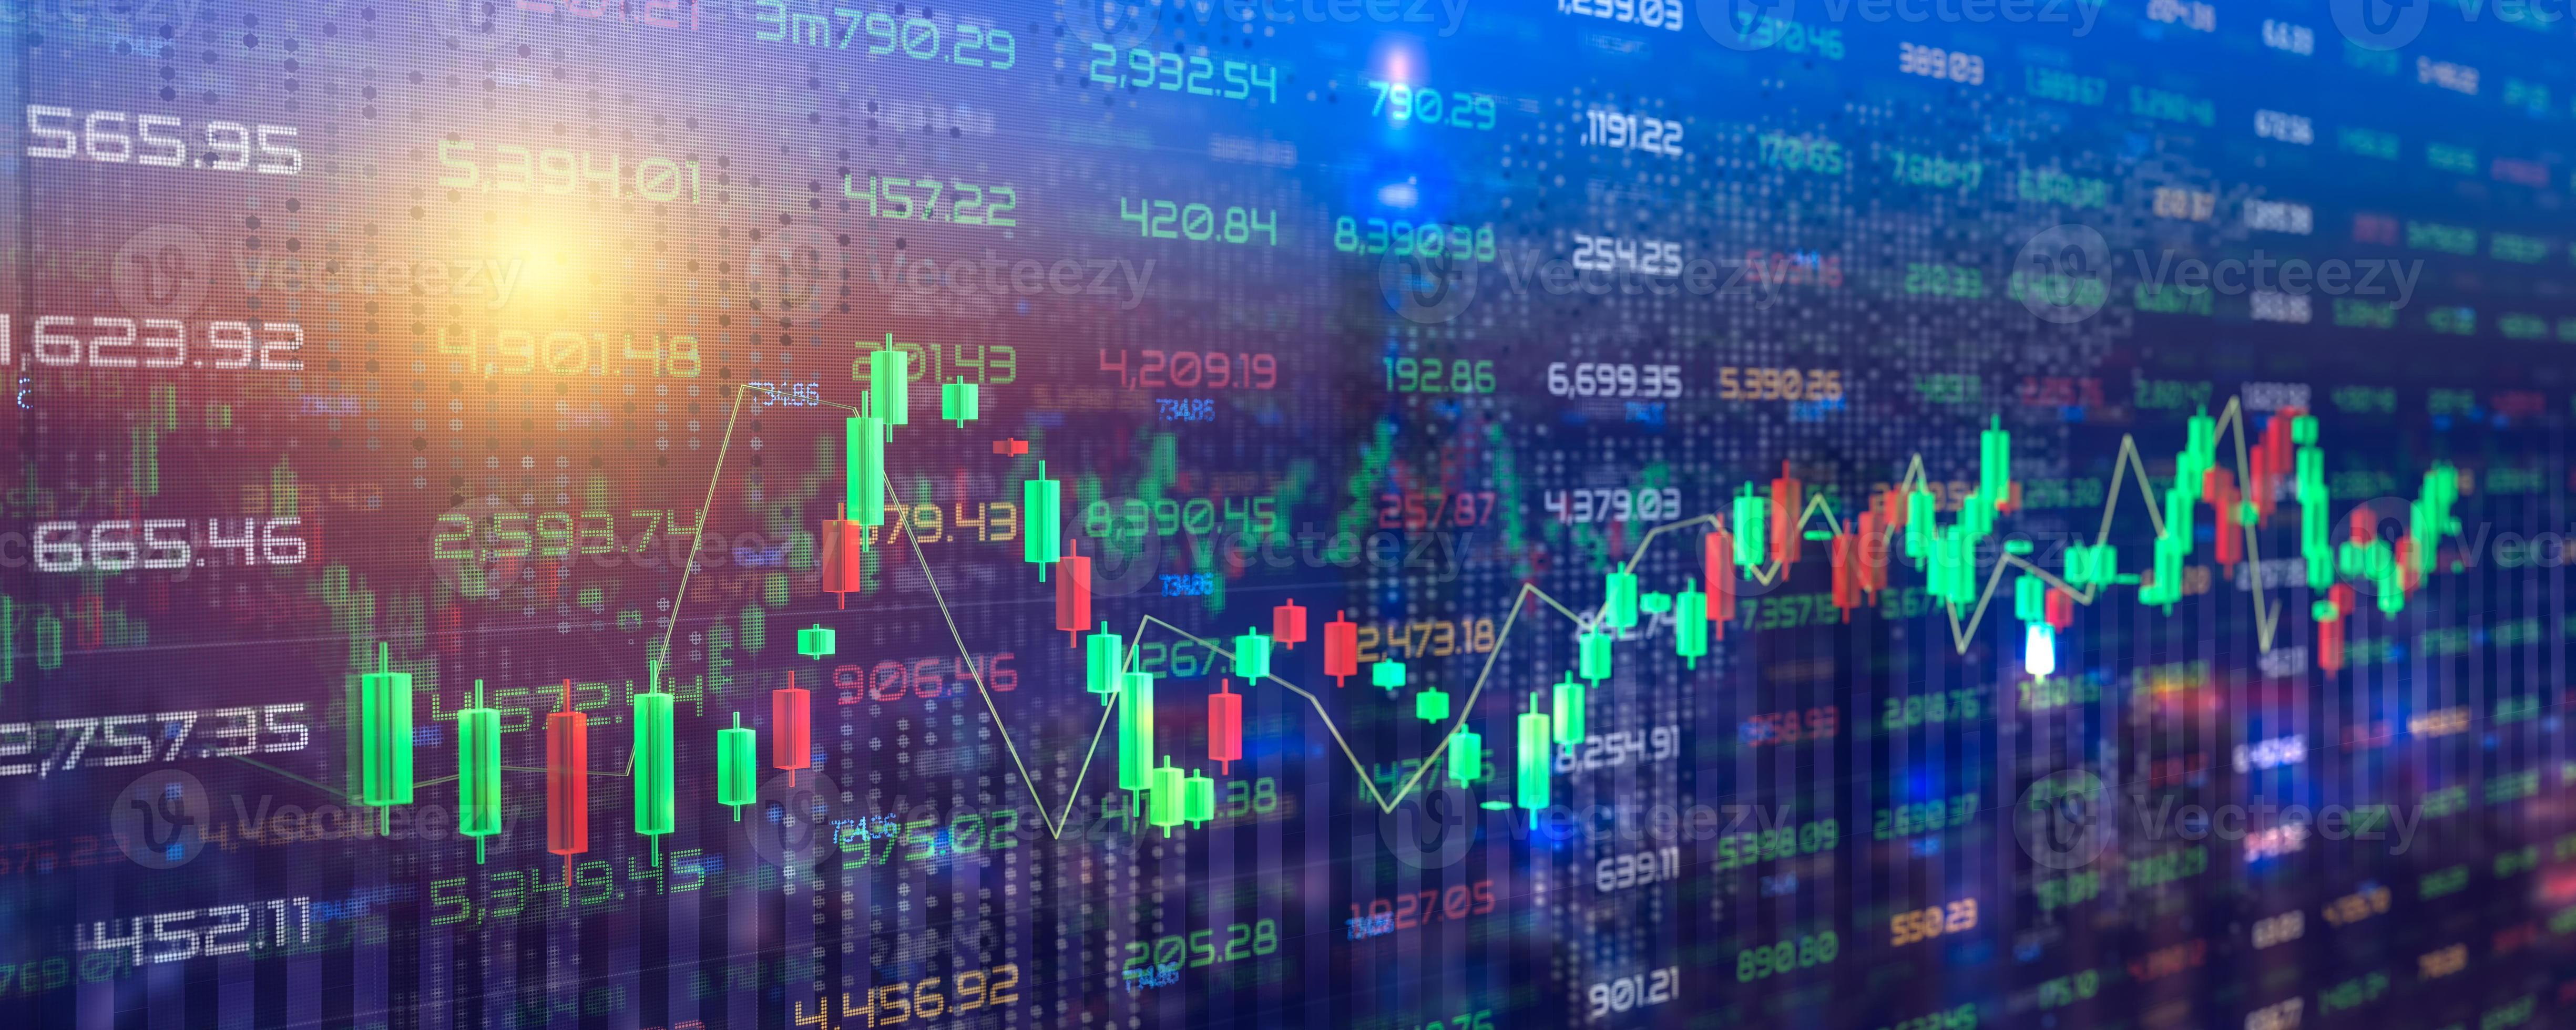
\includegraphics[width=\textwidth,trim=0 780bp 0 780bp,clip]{figures/header_banner.jpg}
  \end{center}
}

% Auto-generated report summary values.
\newcommand{\FilteredArticleCount}{112,807}
\newcommand{\ESGArticleCount}{22,965}
\newcommand{\PanelRows}{5,852}
\newcommand{\PanelTickers}{14}
\newcommand{\PanelStart}{2016-01-01}
\newcommand{\PanelEnd}{2023-12-29}
\newcommand{\NewsWeeks}{2,748}
\newcommand{\BestRegRMSE}{0.0063}
\newcommand{\BestRegRSq}{0.524}
\newcommand{\BestClfAUC}{0.914}
\newcommand{\PriceOnlyAUC}{0.912}
\newcommand{\PriceOnlyRMSE}{0.0064}


\begin{document}

\title{ESG News Risk Forecaster: Predicting Equity Downside Risk from Financial News and Domain-Specific Language Models}

\ifusingacmart
  \author{Ishaan Tibdewal}
  \affiliation{%
    \institution{University of California, San Diego}
    \city{La Jolla}
    \state{California}
    \country{USA}}
  \email{itibdewal@ucsd.edu}
\else
  \author{Ishaan Tibdewal\\University of California, San Diego}
  \date{}
\fi

\ifusingacmart
  \begin{teaserfigure}
    \headervisual
    \vspace{-1.1em}
  \end{teaserfigure}
  \begin{abstract}
  This paper studies whether ESG-sensitive financial news representations improve short-horizon equity risk forecasting beyond market-only baselines. We construct a weekly ticker panel from FNSPID news and price histories, then combine ESG keyword counts, FinBERT sentiment, ClimateBERT climate relevance, and past-only market features. The primary tasks are 21-trading-day realized volatility regression and high-volatility classification, evaluated with chronological train, validation, and test splits. Price-history models are strong, reaching 0.0064 RMSE and 0.912 ROC-AUC on 2023 test weeks after tuning. The best selected configuration is price plus ClimateBERT, with 0.0063 RMSE, $R^2=0.524$, and 0.914 ROC-AUC. The results suggest that ESG text is not a substitute for market features, but climate-aware language signals can add modest incremental value when used as part of a disciplined risk-forecasting pipeline.
  \end{abstract}
  \keywords{ESG, financial news, volatility forecasting, risk prediction, FinBERT, ClimateBERT, FNSPID}
  \maketitle
\else
  \twocolumn[{%
    \maketitle
    \vspace{-0.4em}
    \headervisual
    \vspace{-0.8em}
    \begin{abstract}
    This paper studies whether ESG-sensitive financial news representations improve short-horizon equity risk forecasting beyond market-only baselines. We construct a weekly ticker panel from FNSPID news and price histories, then combine ESG keyword counts, FinBERT sentiment, ClimateBERT climate relevance, and past-only market features. The primary tasks are 21-trading-day realized volatility regression and high-volatility classification, evaluated with chronological train, validation, and test splits. Price-history models are strong, reaching 0.0064 RMSE and 0.912 ROC-AUC on 2023 test weeks after tuning. The best selected configuration is price plus ClimateBERT, with 0.0063 RMSE, $R^2=0.524$, and 0.914 ROC-AUC. The results suggest that ESG text is not a substitute for market features, but climate-aware language signals can add modest incremental value when used as part of a disciplined risk-forecasting pipeline.
    \end{abstract}
    \keywords{ESG, financial news, volatility forecasting, risk prediction, FinBERT, ClimateBERT, FNSPID}
    \vspace{0.2em}
  }]
\fi

\section{Introduction}
Equity risk is affected by more than historical prices. ESG controversies, climate transition risk, governance failures, regulatory shocks, labor disputes, cyber incidents, and sustainability-related events can change investor expectations about cash flows, legal exposure, financing costs, and future uncertainty. These risks are often first observed in textual data: financial news reports, summaries, and public disclosures may reveal operational stress or reputational damage before it is fully reflected in historical return features.

At the same time, market-only baselines are difficult to beat. Recent returns, realized volatility, drawdowns, liquidity, beta, and benchmark co-movement already summarize a large amount of public information. A useful ESG news model therefore should not merely show that news is correlated with risk; it should test whether text-derived features add predictive value beyond price-history features under a time-aware evaluation design.

This project asks the following research question: \emph{Can ESG-sensitive news representations improve short-horizon stock-risk forecasting compared with market-only baselines?} The study is motivated by ESG risk forecasting research such as ESG2Risk \cite{guo2020esg2risk}, but it is implemented as an independent applied machine learning pipeline over FNSPID financial news \cite{dong2024fnspid}, domain-specific language models, and weekly equity-risk targets.

The paper makes four contributions. First, it builds a reproducible weekly modeling panel that aligns financial news, ESG keyword signals, transformer-derived text scores, and daily price histories without loading the full raw news file into memory. Second, it compares market-only, news-only, ESG keyword, FinBERT, ClimateBERT, and combined feature groups for both regression and classification. Third, it uses chronological train, validation, and test periods to reduce lookahead bias. Fourth, it reports aggregate metrics, ablations, diagnostic plots, risk-ranking quintiles, and limitations that clarify when ESG text appears useful.

\section{Related Work}
\subsection{ESG News and Volatility}
The closest conceptual motivation is ESG2Risk, which studies the predictive value of ESG-related financial news for future stock volatility \cite{guo2020esg2risk}. That work frames ESG news as an alternative data source for risk estimation and motivates ranking stocks by predicted risk. This project follows the general research direction but uses a different implementation: weekly feature aggregation, classical and ensemble machine learning models, FNSPID data, FinBERT sentiment, and ClimateBERT relevance rather than a direct reproduction of the original framework.

\subsection{Financial and Climate LMs}
General pretrained language models such as BERT provide contextual representations that improve many NLP tasks \cite{devlin2019bert}. Financial language requires domain awareness because ordinary sentiment words can carry different meanings in finance. FinBERT adapts BERT-style modeling to financial sentiment analysis \cite{araci2019finbert}. ClimateBERT similarly adapts language modeling to climate-related text, improving the detection of climate-relevant language \cite{webersinke2022climatebert}. This project uses these models as feature extractors rather than as end-to-end forecasting architectures.

\subsection{Text, Market Risk, and Tools}
Prior work on financial text shows that disclosures and domain-specific dictionaries can predict risk and market outcomes \cite{kogan2009risk,loughran2011liability}. Climate finance research also suggests that climate news can be priced and hedged in financial markets \cite{engle2020hedging}. The implementation relies on FNSPID for aligned news and prices \cite{dong2024fnspid}, scikit-learn for supervised models \cite{pedregosa2011scikit}, Hugging Face Transformers for model inference \cite{wolf2020transformers}, and yfinance as a relevant market-data tool in the broader project context \cite{aroussi2024yfinance}. XGBoost is included as a project dependency and a natural extension for tree boosting, although the reported pipeline outputs use scikit-learn random forests and gradient boosting models \cite{chen2016xgboost}.

\section{Data and Exploratory Analysis}
\subsection{News and Price Sources}
The repository uses FNSPID, a financial news and stock price integration dataset that combines financial news records with price histories \cite{dong2024fnspid}. The local raw data contains a 23.23 GB file, \texttt{nasdaq\_external\_data.csv}, with dates, article titles, stock symbols, URLs, publishers, authors, full article text, and extractive summaries. The local price directory contains 7,693 ticker-level CSV files. Tables~\ref{tab:dataset-summary} and~\ref{tab:ticker-universe} summarize the filtered data, modeled universe, and final weekly panel.

\begin{table}[t]
  \caption{Dataset and modeling panel summary.}
  \label{tab:dataset-summary}
  \centering
  \small
  \setlength{\tabcolsep}{3pt}
  \begin{tabular}{@{}p{0.58\columnwidth}r@{}}
    \toprule
    Quantity & Value \\
    \midrule
    Raw FNSPID news file size & 23.23 GB \\
    Available price-history files & 7,693 \\
    Filtered news articles & 112,807 \\
    ESG keyword-matched articles & 22,965 \\
    News date range & 2010-02-17--2023-12-31 \\
    Modeled tickers & 14 \\
    Average articles per modeled ticker & 8,057.6 \\
    Final weekly modeling rows & 5,852 \\
    ESG/news ticker-weeks & 2,748 \\
    Panel date range & 2016-01-01--2023-12-29 \\
    Benchmark & QQQ \\
    \bottomrule
  \end{tabular}
\end{table}

\begin{table}[t]
  \caption{Modeled ticker universe and filtered-news coverage.}
  \label{tab:ticker-universe}
  \centering
  \small
  \setlength{\tabcolsep}{4pt}
  \begin{tabular}{lrlr}
    \toprule
    Ticker & Articles & Ticker & Articles \\
    \midrule
    AAPL & 9,338 & JNJ & 2,928 \\
    AMD & 9,139 & JPM & 2,863 \\
    AMZN & 5,060 & MSFT & 8,737 \\
    COST & 6,781 & NVDA & 11,862 \\
    CVX & 8,688 & TSLA & 10,587 \\
    DIS & 9,651 & WMT & 8,686 \\
    INTC & 11,141 & XOM & 7,346 \\
    \bottomrule
  \end{tabular}
\end{table}


The modeled universe contains 14 large, liquid, news-covered equities. The final modeling panel has \PanelRows{} ticker-week rows across \PanelTickers{} tickers from \PanelStart{} to \PanelEnd{}. The benchmark is QQQ because it is available in the FNSPID price histories through the test period. The pipeline initially considered additional large-cap tickers, but excludes tickers whose price coverage does not reach the 2023 test period.

\subsection{Filtering, Cleaning, and Alignment}
The raw news file is too large to load naively, so the pipeline performs bounded schema inspection and chunked filtering by ticker and date. Text features are built from article titles and available summaries or article text. Articles are normalized to ticker-date records and then aligned to week-ending Friday dates. Price histories are cleaned into daily adjusted close, volume, and one-day return records. Weekly feature rows are created by taking the last available market feature within each ticker-week and by aggregating article-level news signals to ticker-week features.

Missing text features arise naturally because not every ticker has ESG-related news every week. The final panel therefore distinguishes all test weeks from ESG/news test weeks. This distinction is important: text features should not be credited or penalized in the same way on weeks with no relevant article coverage.

\subsection{Exploratory Findings}
Figures~\ref{fig:coverage-overview} and~\ref{fig:text-target-distributions} highlight several properties that shape the modeling design. News coverage is uneven across tickers and over time, so a ticker-week panel must distinguish weeks with ESG/news coverage from weeks with no matched articles. ESG keyword matching provides an interpretable first screen for environmental, social, governance, and controversy language, but it is noisy because keyword mentions do not always imply material firm-level risk. FinBERT sentiment is broadly distributed, suggesting that article tone contains variation beyond simple article counts. The future volatility target is right-skewed, which motivates reporting both regression errors and high-risk classification or ranking diagnostics.

\begin{figure*}[t]
  \centering
  \begin{subfigure}[t]{0.64\textwidth}
    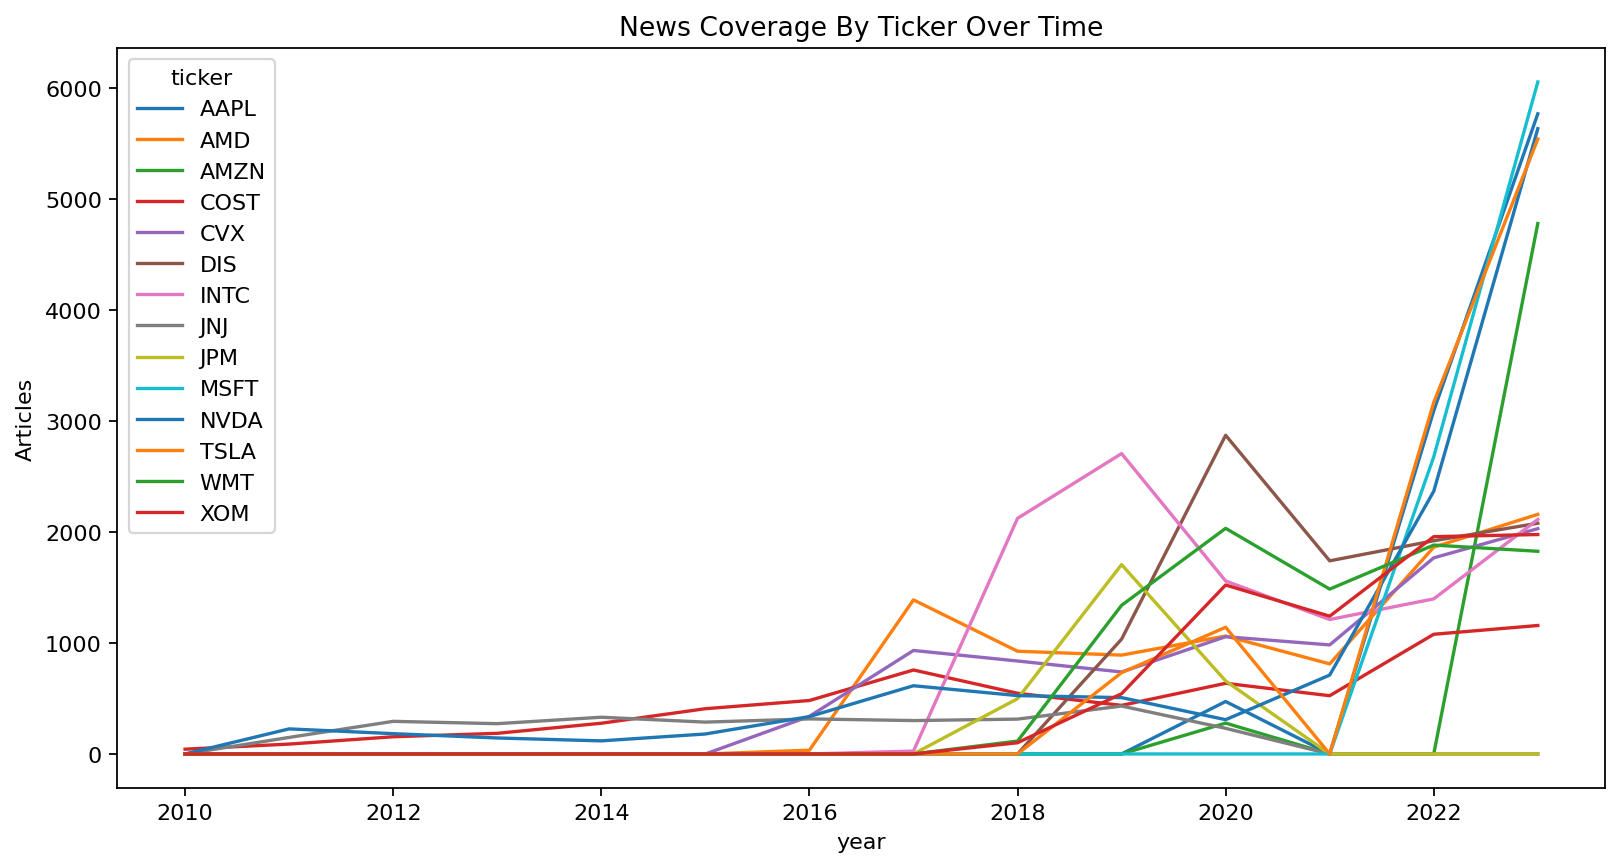
\includegraphics[width=\linewidth]{figures/dataset_distribution.png}
    \caption{News coverage}
  \end{subfigure}
  \hfill
  \begin{subfigure}[t]{0.32\textwidth}
    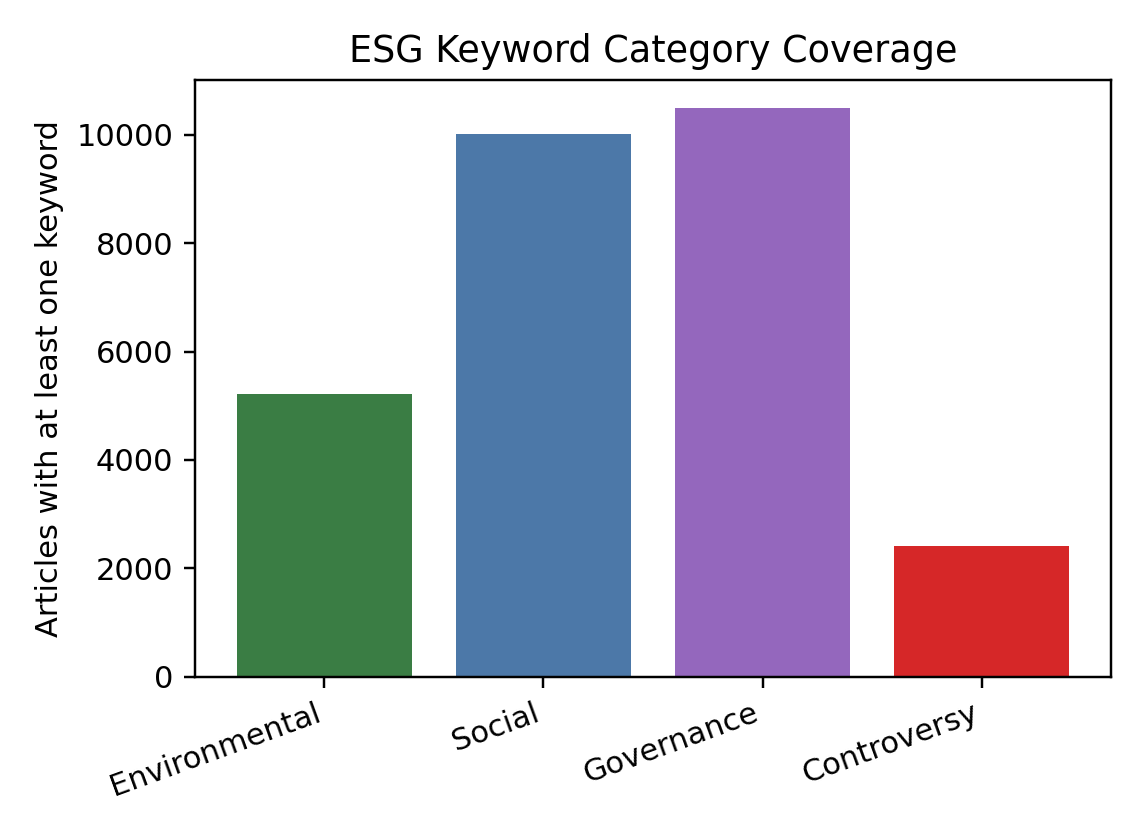
\includegraphics[width=\linewidth]{figures/esg_category_distribution.png}
    \caption{ESG categories}
  \end{subfigure}
  \caption{Coverage diagnostics for the modeling panel. News volume is uneven across firms and years, and ESG keyword categories provide an interpretable but noisy screen for article relevance.}
  \label{fig:coverage-overview}
  \Description{Two-panel figure summarizing news coverage and ESG category counts.}
\end{figure*}

\begin{figure*}[t]
  \centering
  \begin{subfigure}[t]{0.49\textwidth}
    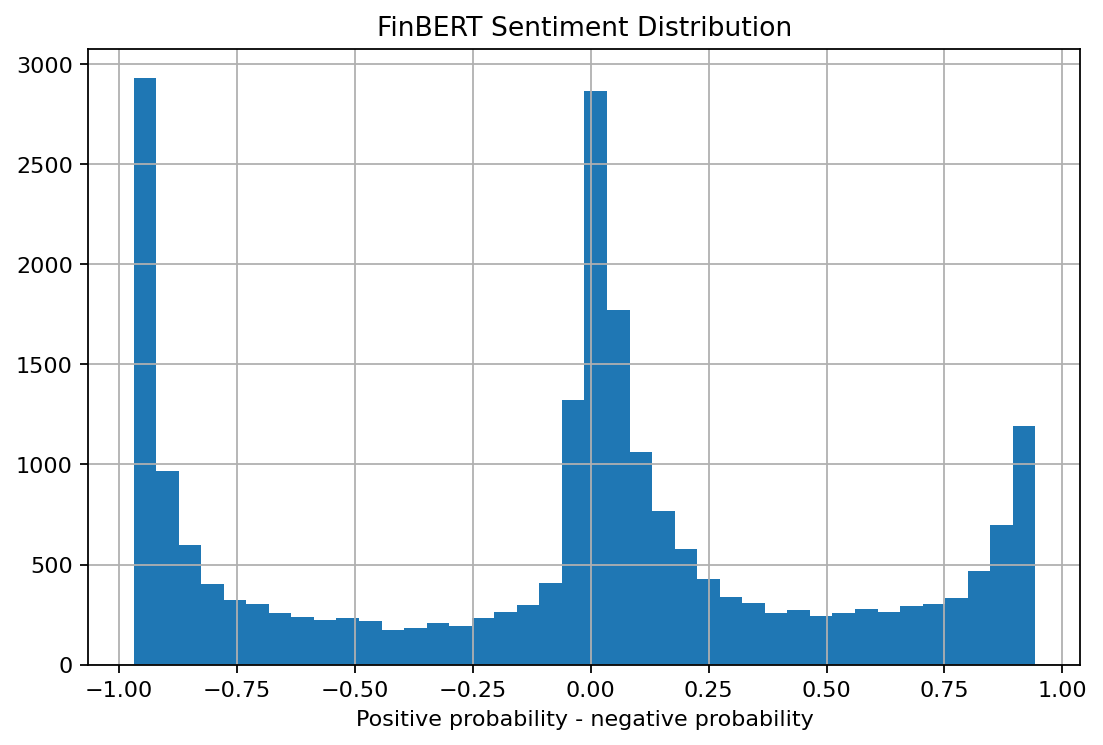
\includegraphics[width=\linewidth]{figures/sentiment_distribution.png}
    \caption{FinBERT sentiment}
  \end{subfigure}
  \hfill
  \begin{subfigure}[t]{0.49\textwidth}
    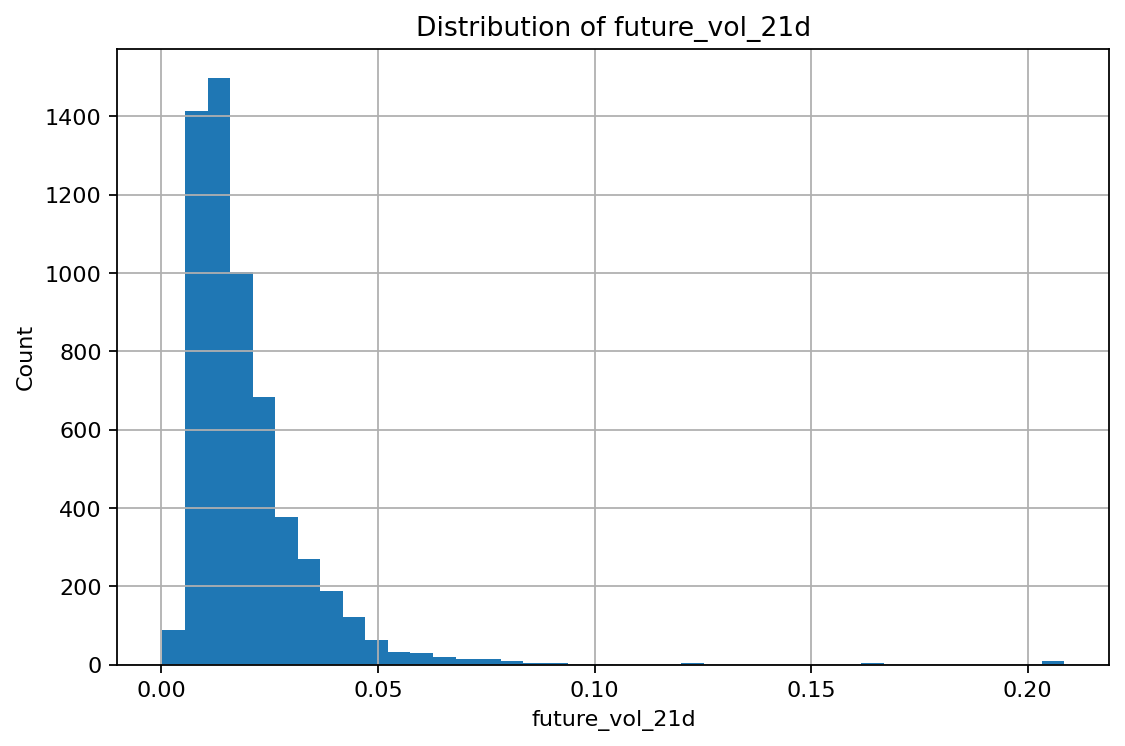
\includegraphics[width=\linewidth]{figures/risk_label_distribution.png}
    \caption{Risk target}
  \end{subfigure}
  \caption{Text-signal and target diagnostics. FinBERT sentiment has broad variation across articles, while the realized-volatility target is right-skewed.}
  \label{fig:text-target-distributions}
  \Description{Two-panel figure summarizing FinBERT sentiment and realized volatility target distributions.}
\end{figure*}

\FloatBarrier
\section{Predictive Task and Evaluation Design}
The supervised input unit is a ticker-week observation $(i,t)$: all available past-only market features and same-week aggregated news features for ticker $i$ are used to predict future risk after week $t$. The main baseline is a price-history-only model. This is an appropriate and strong baseline because realized volatility is persistent, and recent returns, drawdowns, volume, beta, and benchmark co-movement already summarize substantial public market information. ESG/news features may still add value when textual reports reveal climate exposure, regulatory pressure, operational disruptions, or reputational risk not fully captured by trailing prices.

\subsection{Prediction Tasks}
Task 1 is 21-trading-day realized volatility regression. The target is
\begin{equation}
  y_{i,t}^{\mathrm{vol}} =
  \sqrt{\frac{1}{H}\sum_{k=1}^{H} r_{i,t+k}^{2}},
  \quad H=21,
  \label{eq:future-vol}
\end{equation}
where $r_{i,t+k}$ is the future daily return. Task 2 is high-volatility classification. The label marks ticker-weeks whose future volatility falls in the top quartile within the same week:
\begin{equation}
  y_{i,t}^{\mathrm{high}} =
  \mathbb{1}\{y_{i,t}^{\mathrm{vol}} \ge Q_{0.75,t}(y^{\mathrm{vol}})\}.
  \label{eq:high-vol}
\end{equation}
The within-week threshold makes the classification task a cross-sectional risk-screening problem rather than a single global thresholding exercise.

\subsection{Chronological Split and Metrics}
The chronological split is 2016--2021 for training, 2022 for validation and hyperparameter selection, and 2023 for final testing. This avoids training on future market regimes and supports validation-based model tuning before the held-out test year. Regression is evaluated with RMSE, MAE, $R^2$, and Spearman rank correlation. Classification is evaluated with ROC-AUC, PR-AUC, F1, precision, recall, confusion matrices, and precision at the top 10 percent of predicted risk. The report also uses predicted-risk quintiles to evaluate whether higher predicted risk corresponds to higher realized volatility.

\section{Methodology}
\subsection{Pipeline Overview}
Figure~\ref{fig:pipeline} summarizes the end-to-end pipeline. The system combines news ingestion, ESG keyword filtering, transformer scoring, weekly aggregation, market feature engineering, target construction, model fitting, and evaluation.

\begin{figure*}[t]
  \centering
  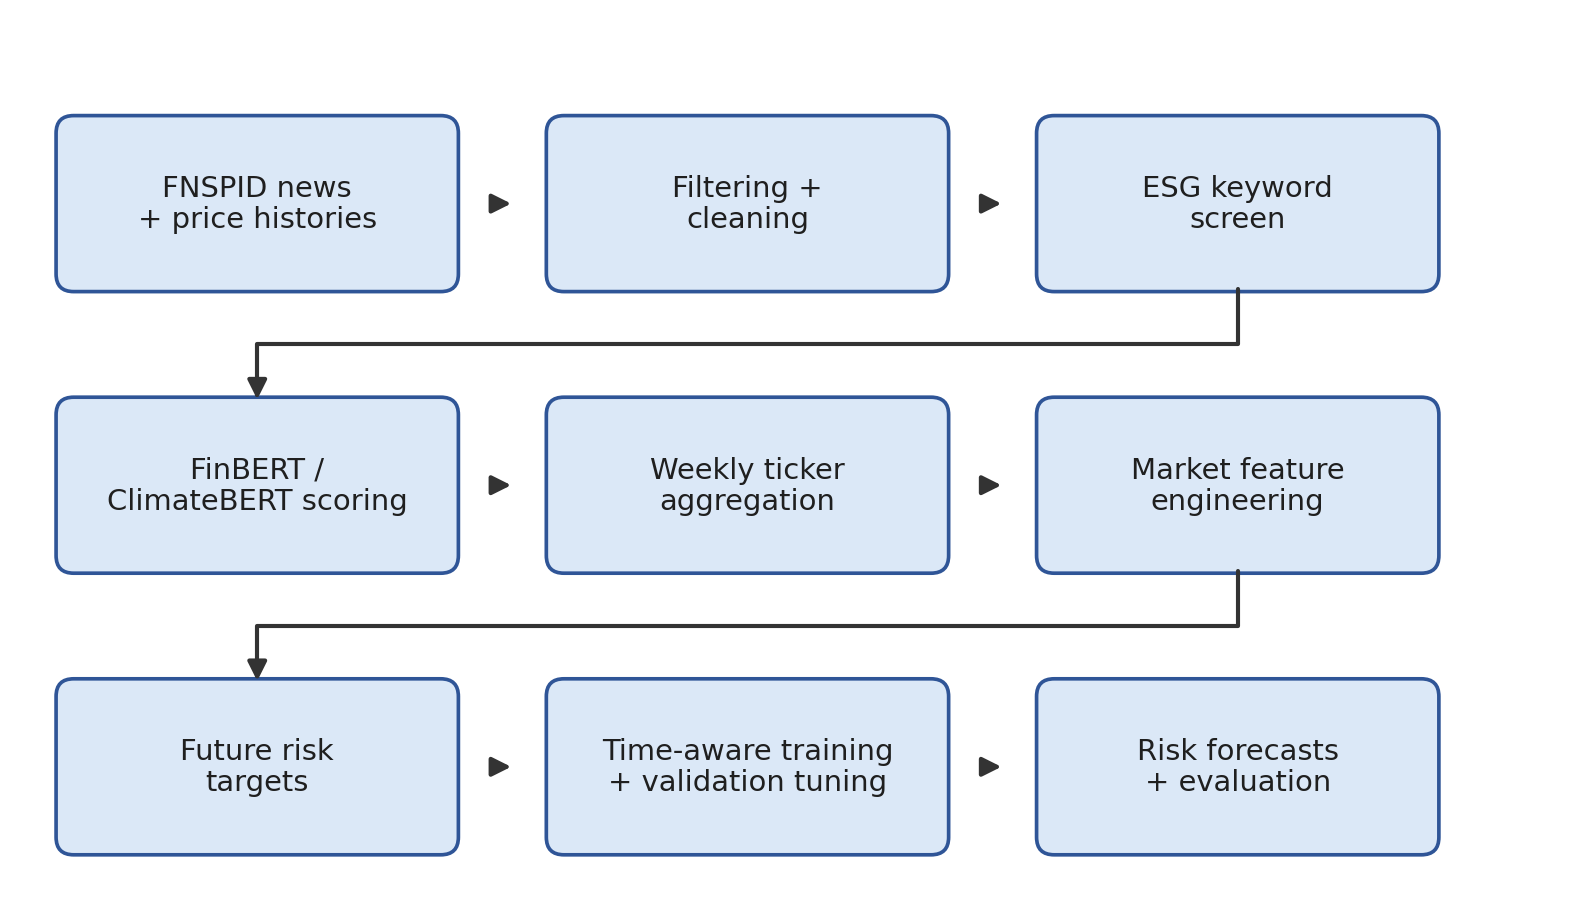
\includegraphics[width=0.84\textwidth,height=0.28\textheight,keepaspectratio]{figures/pipeline_overview.png}
  \caption{Project pipeline from FNSPID news and price histories to weekly risk forecasts: filtering and cleaning, ESG keyword screening, FinBERT and ClimateBERT scoring, weekly aggregation, market feature engineering, target construction, model training, and evaluation.}
  \label{fig:pipeline}
  \Description{Flow diagram showing preprocessing, language model features, aggregation, market features, labels, training, and evaluation.}
\end{figure*}

\subsection{Market Features}
Daily simple returns are computed from adjusted close prices:
\begin{equation}
  r_{i,d} = \frac{P_{i,d}}{P_{i,d-1}} - 1,
  \label{eq:return}
\end{equation}
where $P_{i,d}$ is the adjusted close for ticker $i$ on day $d$. Past-only price features include trailing returns, rolling volatility, rolling drawdown, distance from moving averages and 52-week highs, rolling average volume, volume surprise, benchmark excess return, rolling beta, and rolling correlation. For example, rolling volatility over a past window $h$ is
\begin{equation}
  \widehat{\sigma}_{i,d,h}^{\mathrm{past}} =
  \sqrt{\frac{1}{h-1}\sum_{j=0}^{h-1}(r_{i,d-j}-\bar{r}_{i,d,h})^2}.
  \label{eq:rolling-vol}
\end{equation}

\subsection{News and Language Features}
The ESG keyword stage counts environmental, social, governance, and controversy keyword matches in cleaned article text. Article-level indicators are aggregated to ticker-week counts, shares, and intensities. For a generic article signal $s_{i,a}$ associated with ticker $i$ and week $t$, the weekly average feature is
\begin{equation}
  x_{i,t}^{\mathrm{text}} =
  \frac{1}{|A_{i,t}|}\sum_{a \in A_{i,t}} s_{i,a},
  \label{eq:aggregation}
\end{equation}
where $A_{i,t}$ is the set of articles for ticker $i$ in week $t$.

FinBERT features use the ProsusAI FinBERT model to estimate positive, neutral, and negative financial sentiment probabilities \cite{araci2019finbert}. The pipeline derives a sentiment score as positive probability minus negative probability and aggregates average, minimum, maximum, volatility, negative share, and lagged sentiment signals. ClimateBERT features use a DistilRoBERTa-based climate detector to estimate climate relevance \cite{webersinke2022climatebert}. Climate relevance, climate article share, climate intensity, and interactions with negative FinBERT sentiment are aggregated weekly.

\subsection{Model Families and Preprocessing}
For regression, models learn a function $f_\theta(x_{i,t})$ by minimizing squared prediction error over the training period:
\begin{equation}
  \min_{\theta} \sum_{(i,t)\in \mathcal{T}_{\mathrm{train}}}
  \left(y_{i,t}^{\mathrm{vol}} - f_\theta(x_{i,t})\right)^2.
  \label{eq:objective}
\end{equation}
For classification, models estimate a high-risk probability $\hat{p}_{i,t}=g_\theta(x_{i,t})$. Regression models include Ridge regression, random forest regression, gradient boosting regression, and histogram gradient boosting regression. Classification models include logistic regression, random forest classification, gradient boosting classification, and histogram gradient boosting classification. Numeric features are median-imputed; Ridge and logistic regression are scaled.

\section{Experiments}
\subsection{Feature Groups and Baselines}
The experiment compares market-only, text-only, and combined feature groups. Market-only features are the main baseline. News-only groups include ESG keyword, FinBERT, ClimateBERT, and all-news features. Combined groups include price plus keyword, price plus FinBERT, price plus ClimateBERT, price plus FinBERT plus ClimateBERT, price plus all news, and a full group that includes all available numeric features. Table~\ref{tab:experiment-matrix} summarizes the main comparison; price plus ClimateBERT is the best selected combined configuration in the tuned 2023 test results.

\begin{table*}[t]
  \caption{Experiment feature groups compared in the study.}
  \label{tab:experiment-matrix}
  \centering
  \small
  \setlength{\tabcolsep}{4pt}
  \begin{tabularx}{\textwidth}{@{}>{\raggedright\arraybackslash}p{0.14\textwidth}X>{\raggedright\arraybackslash}p{0.24\textwidth}@{}}
    \toprule
    Group & Feature content & Purpose \\
    \midrule
    Price & Returns, volatility, drawdown, volume, beta/correlation & Main market-only baseline \\
    ESG keyword & ESG and controversy keyword counts & Interpretable text-only ESG screen \\
    FinBERT & Sentiment probabilities and aggregates & Test financial tone signal \\
    ClimateBERT & Climate relevance and intensity aggregates & Test climate-specific signal \\
    Price + ClimateBERT & Market features plus ClimateBERT aggregates & Best selected combined configuration \\
    Price + All News & Market features plus all text features & Broad price-plus-text ablation \\
    Full & All available numeric features & Upper-bound combined feature set \\
    \bottomrule
  \end{tabularx}
\end{table*}

\subsection{Models and Hyperparameters}
Hyperparameters are selected on the 2022 validation set and refit on train plus validation before testing on 2023. Validation grids include linear regularization strength, random forest leaf size and feature subsampling, and boosting learning rate, depth, iteration count, leaf count, and $L_2$ regularization. Table~\ref{tab:hyperparams} reports the validation-selected histogram-gradient-boosting hyperparameters for the rows shown in Table~\ref{tab:model-performance}.

\begin{table}[t]
  \caption{Validation-selected hyperparameters for histogram gradient boosting (HGB).}
  \label{tab:hyperparams}
  \centering
  \scriptsize
  \setlength{\tabcolsep}{1.5pt}
  \begin{tabular}{@{}llp{0.48\columnwidth}@{}}
    \toprule
    Task & Group & Selected hyperparameters \\
    \midrule
    Reg. & Price & lr=0.03; iter=100; leaf=15; $L_2$=0.1 \\
    Reg. & Price + ClimateBERT & lr=0.03; iter=100; leaf=15; $L_2$=0.1 \\
    Class. & Price & lr=0.03; iter=200; leaf=15; $L_2$=0.1 \\
    Class. & Price + ClimateBERT & lr=0.05; iter=200; leaf=15; $L_2$=0.1 \\
    \bottomrule
  \end{tabular}
\end{table}

\FloatBarrier
\subsection{Reproducibility}
The project repository is available at
\url{https://github.com/ishaantibdewal/esg-news-risk-forecaster}.
It contains preprocessing, feature generation, model evaluation, generated figures, tables, notebooks, the Streamlit demo script, and this report source. The README describes the main reproduction sequence: run staged pipeline commands for setup, bounded data inspection, chunked news filtering, price-label construction, feature generation, FinBERT and ClimateBERT scoring, panel construction, model evaluation, and report generation.

\section{Results}
\subsection{Overall Performance}
\begin{table*}[t]
  \caption{Best validation-tuned model performance on the 2023 test period. Lower RMSE and MAE are better; higher $R^2$, ROC-AUC, PR-AUC, and F1 are better.}
  \label{tab:model-performance}
  \centering
  \small
  \setlength{\tabcolsep}{4pt}
  \begin{tabular}{lllrrrrrr}
    \toprule
    Task & Feature group & Model & RMSE & MAE & $R^2$ & ROC-AUC & PR-AUC & F1 \\
    \midrule
    Reg. & Price & HGB & 0.0064 & 0.0048 & 0.504 & -- & -- & -- \\
    Reg. & Price + ClimateBERT & HGB & 0.0063 & 0.0047 & 0.524 & -- & -- & -- \\
    Reg. & Price + All News & HGB & 0.0065 & 0.0049 & 0.497 & -- & -- & -- \\
    Reg. & Full & HGB & 0.0065 & 0.0049 & 0.497 & -- & -- & -- \\
    Class. & Price & HGB & -- & -- & -- & 0.912 & 0.841 & 0.798 \\
    Class. & Price + ClimateBERT & HGB & -- & -- & -- & 0.914 & 0.851 & 0.802 \\
    Class. & Price + All News & HGB & -- & -- & -- & 0.913 & 0.836 & 0.777 \\
    Class. & Full & HGB & -- & -- & -- & 0.913 & 0.836 & 0.777 \\
    \bottomrule
  \end{tabular}
\end{table*}

\noindent Table~\ref{tab:model-performance} reports the best validation-tuned models by feature group on the 2023 test period. The strongest selected regression result is price plus ClimateBERT with RMSE \BestRegRMSE{} and $R^2=\BestRegRSq{}$, compared with \PriceOnlyRMSE{} RMSE for price-only. The strongest selected classification result is also price plus ClimateBERT with ROC-AUC \BestClfAUC{}, compared with \PriceOnlyAUC{} for price-only. Because the performance gap between the price-only and price-plus-ClimateBERT models is small, the result should be interpreted as modest incremental evidence rather than a definitive improvement.

\subsection{Ablation Study}
\begin{table}[H]
  \caption{Ablation summary relative to tuned price-only baselines. Positive $\Delta$RMSE means lower error than price-only; positive $\Delta$AUC means higher ROC-AUC than price-only.}
  \label{tab:ablation}
  \centering
  \small
  \setlength{\tabcolsep}{3pt}
  \begin{tabular}{lrrrr}
    \toprule
    Feature group & RMSE & $\Delta$RMSE & AUC & $\Delta$AUC \\
    \midrule
    Price & 0.0064 & 0.0000 & 0.912 & 0.000 \\
    Price + ClimateBERT & 0.0063 & 0.0001 & 0.914 & 0.002 \\
    Price + All News & 0.0065 & 0.0000 & 0.913 & 0.001 \\
    Full & 0.0065 & 0.0000 & 0.913 & 0.001 \\
    \bottomrule
  \end{tabular}
\end{table}

\noindent Table~\ref{tab:ablation} compares tuned combined feature sets against the price-only baseline. News-only models underperform price-only models, indicating that financial text is not sufficient by itself for weekly volatility forecasting. Among combined models, ClimateBERT adds the clearest incremental value in the selected tuned run. The full feature group performs competitively but does not outperform price plus ClimateBERT, suggesting that additional text features can add noise as well as signal.

\subsection{Classification Diagnostics}
Figures~\ref{fig:roc-diagnostic} and~\ref{fig:confusion-diagnostic} show that the selected price and ClimateBERT classifier separates high-volatility weeks well but still makes errors near the risk threshold. This supports using the classifier as a screening model rather than as a standalone decision rule.

\begin{figure}[H]
  \centering
  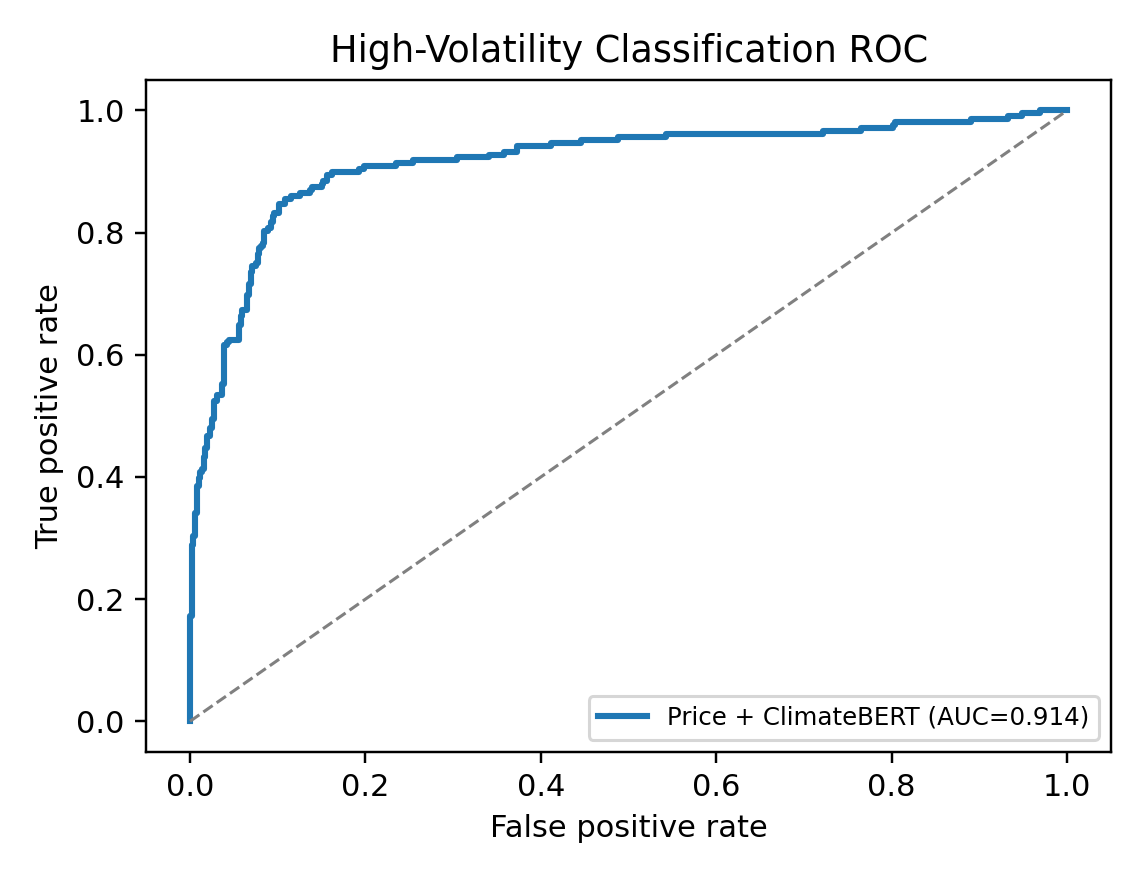
\includegraphics[width=\linewidth]{figures/roc_curve.png}
  \caption{ROC curve for the selected price-plus-ClimateBERT classifier on 2023 test weeks.}
  \label{fig:roc-diagnostic}
  \Description{ROC curve for the selected classifier.}
\end{figure}

\begin{figure}[H]
  \centering
  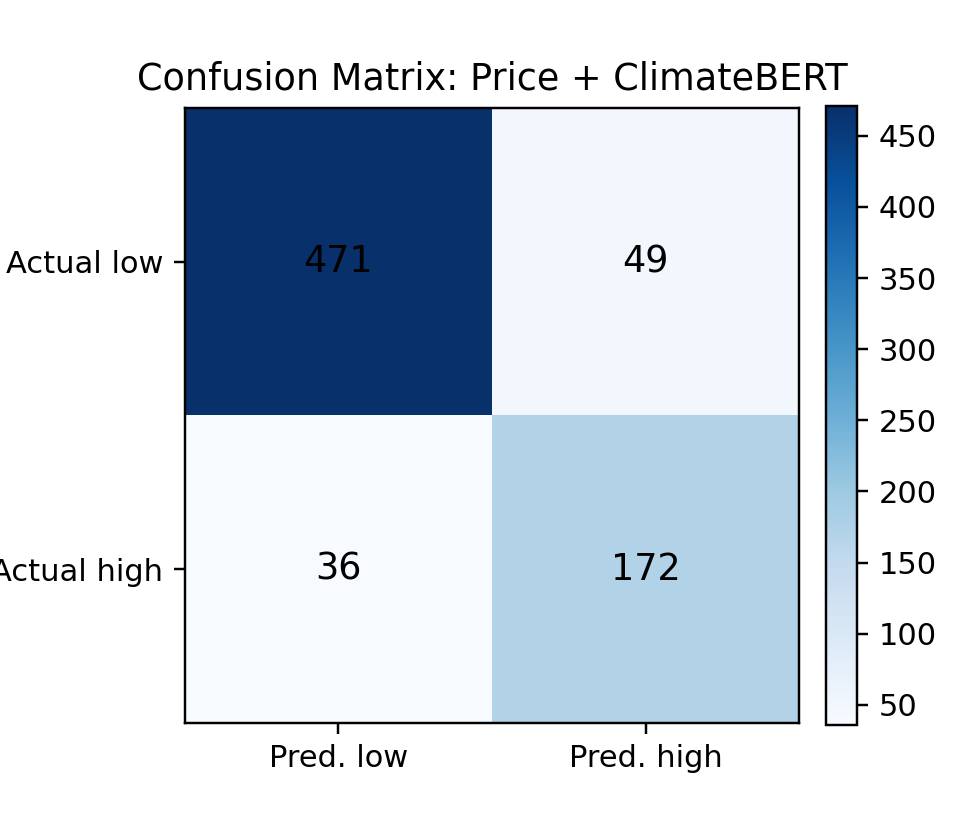
\includegraphics[width=0.92\linewidth]{figures/confusion_matrix.png}
  \caption{Confusion matrix for the selected price-plus-ClimateBERT classifier on 2023 test weeks.}
  \label{fig:confusion-diagnostic}
  \Description{Confusion matrix for the selected classifier.}
\end{figure}

\subsection{Regression and Ranking Diagnostics}
Figures~\ref{fig:predicted-realized-diagnostic} and~\ref{fig:quintile-diagnostic} compare predicted and realized volatility and then group predictions into risk quintiles. The quintile pattern shows that predicted risk is useful for ranking observations even though individual realized-volatility errors remain visible.

\begin{figure}[H]
  \centering
  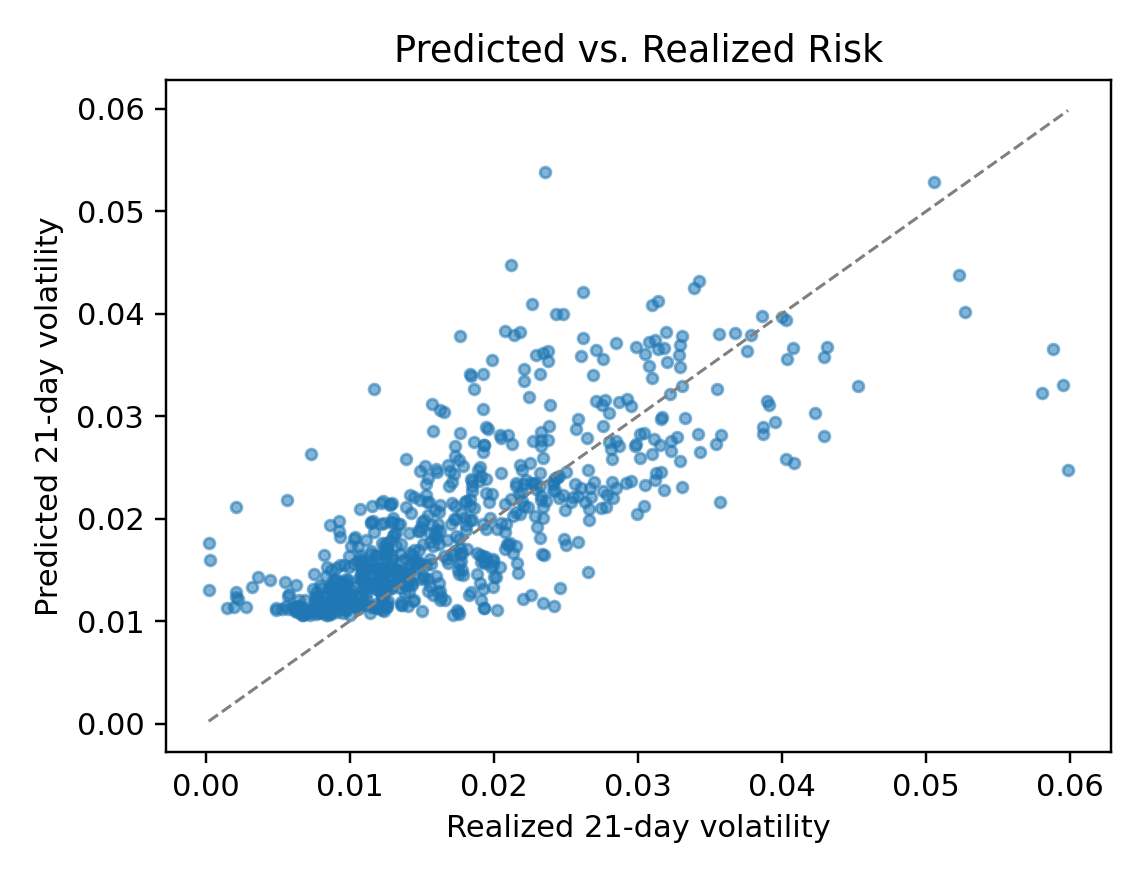
\includegraphics[width=\linewidth]{figures/predicted_vs_realized_risk.png}
  \caption{Predicted versus realized volatility for the selected price-plus-ClimateBERT model on 2023 test weeks.}
  \label{fig:predicted-realized-diagnostic}
  \Description{Predicted versus realized volatility scatterplot.}
\end{figure}

\begin{figure}[H]
  \centering
  
\includegraphics[width=\linewidth]{figures/quintile_realized_volatility.png}
  \caption{Realized volatility by predicted-risk quintile for the selected price-plus-ClimateBERT model on 2023 test weeks.}
  \label{fig:quintile-diagnostic}
  \Description{Bar chart of realized volatility by predicted-risk quintile.}
\end{figure}

\subsection{Feature and Error Diagnostics}
Figures~\ref{fig:feature-diagnostic} and~\ref{fig:ticker-diagnostic} summarize feature associations and a selected ticker-level time series. The diagnostics show that market variables remain dominant, while climate-aware text signals contribute as secondary predictors in the combined model.

\begin{figure}[H]
  \centering
  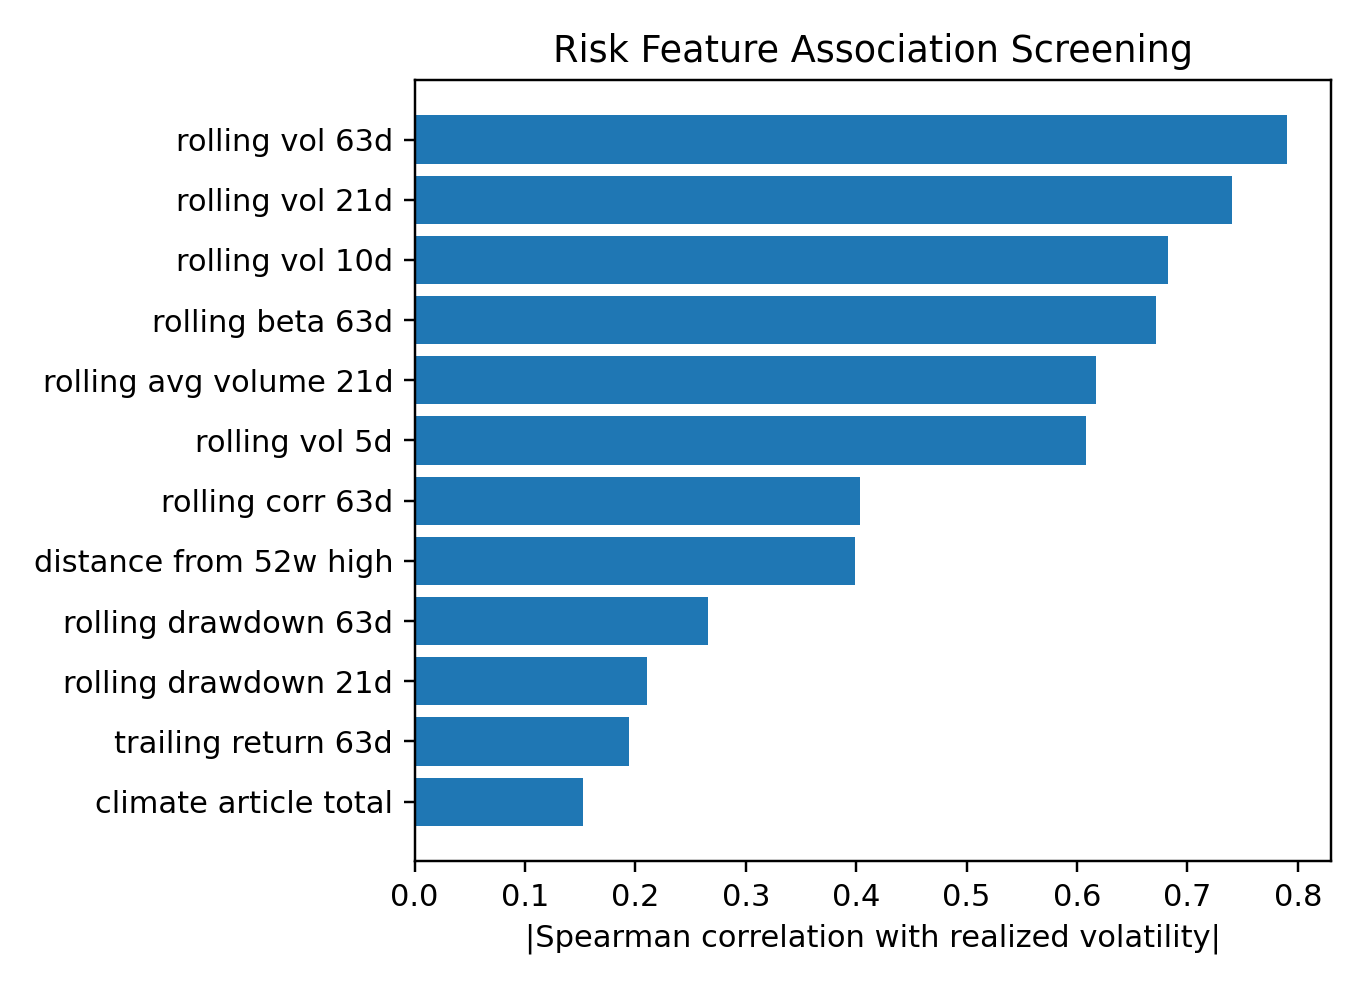
\includegraphics[width=\linewidth]{figures/feature_importance.png}
  \caption{Top feature associations for the selected price-plus-ClimateBERT model.}
  \label{fig:feature-diagnostic}
  \Description{Feature association chart for the selected model.}
\end{figure}

\begin{figure}[H]
  \centering
  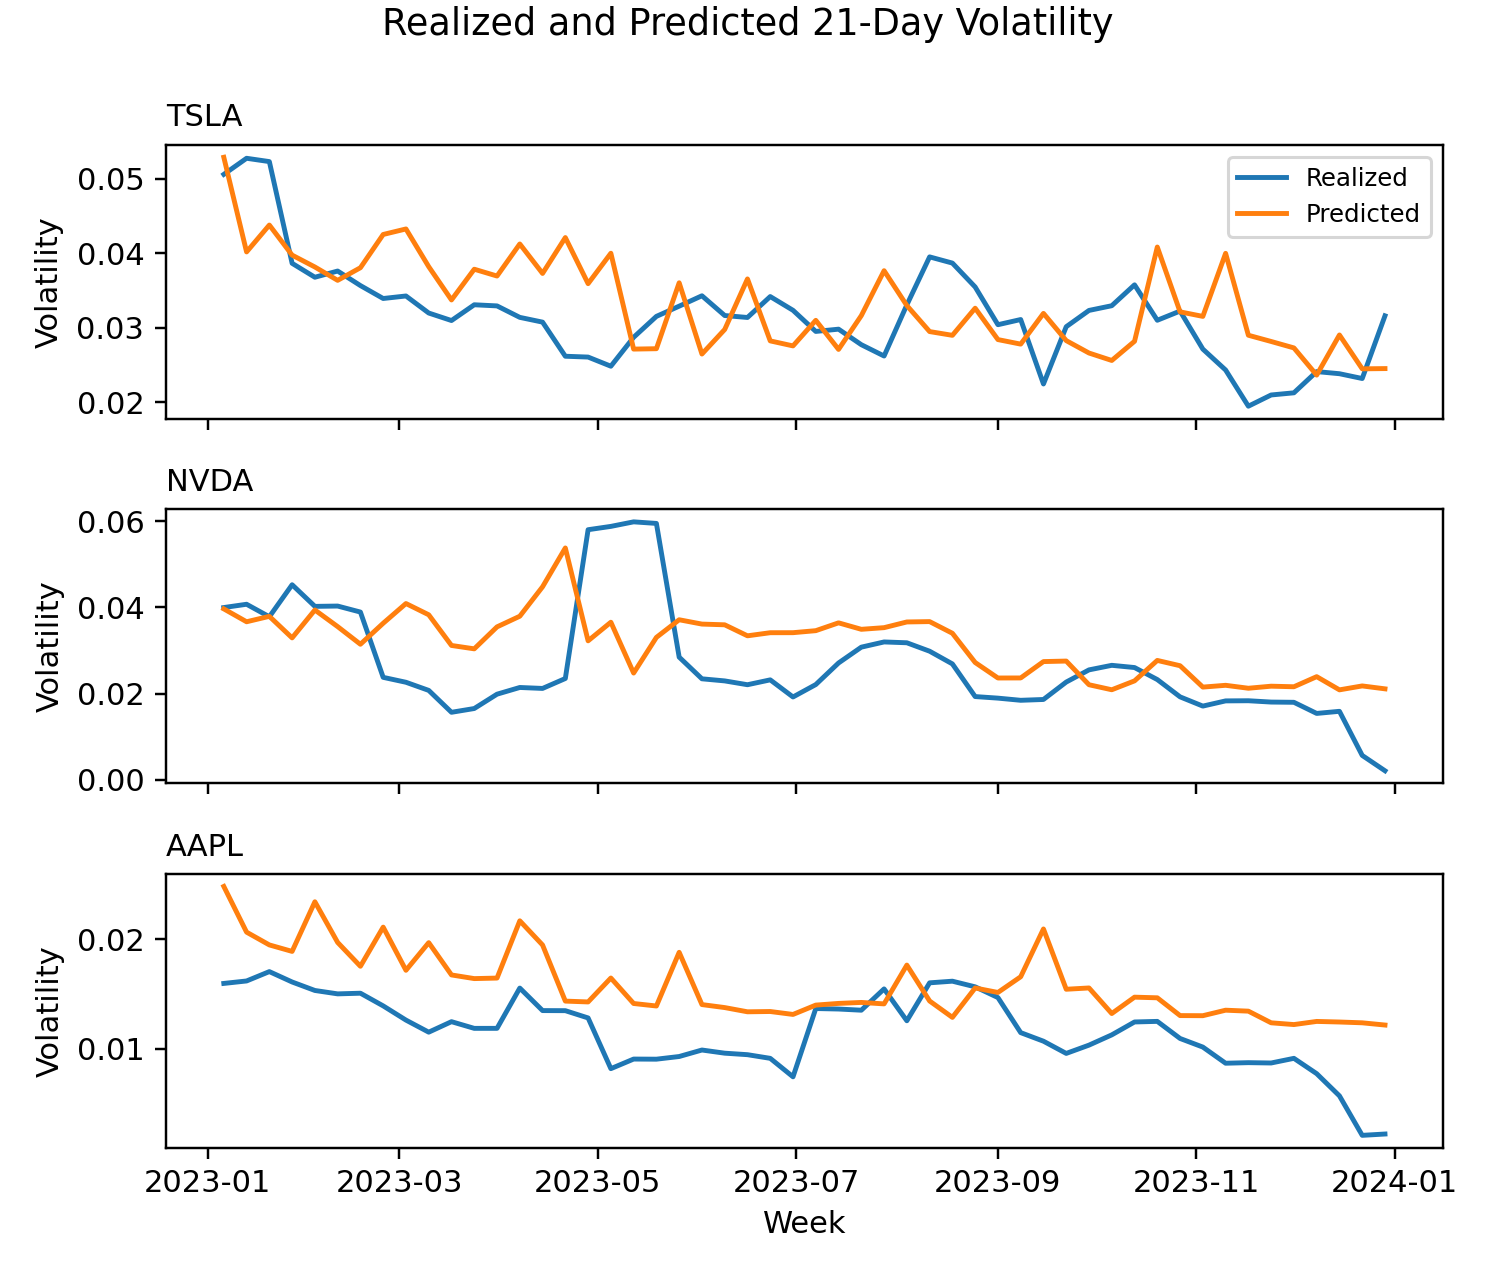
\includegraphics[width=\linewidth]{figures/timeseries_predicted_realized_risk.png}
  \caption{Selected ticker-level predicted and realized volatility time series for 2023 test weeks.}
  \label{fig:ticker-diagnostic}
  \Description{Ticker-level predicted-versus-realized volatility time series.}
\end{figure}

\FloatBarrier
\section{Discussion}
The results indicate that ESG-sensitive text features can help, but only under a careful interpretation. Price-only baselines are strong because volatility is persistent and because recent drawdowns, beta, volume, and benchmark correlation already encode substantial market information. This makes the marginal contribution of text difficult to isolate. The diagnostics in Figures~\ref{fig:roc-diagnostic}--\ref{fig:ticker-diagnostic} summarize the main empirical patterns behind this conclusion.

The strongest positive result is the tuned price-plus-ClimateBERT configuration. Climate relevance may be more targeted than broad ESG keyword counts or general financial sentiment because climate risk captures regulatory, transition, physical, and reputation concerns that can affect future uncertainty. By contrast, keyword counts are interpretable but noisy, and FinBERT sentiment alone may not distinguish news that changes volatility from news that merely has positive or negative tone.

The weaker performance of news-only models is also informative. News coverage is sparse and uneven across ticker-weeks, and some weeks have no relevant ESG articles. Text signals appear most useful as complements to market features rather than replacements. This supports a sustainable-investing research workflow in which language models enrich existing risk models rather than operate as standalone trading signals.

\section{Limitations}
Several limitations constrain the conclusions. First, the ticker universe is small and biased toward large, news-covered equities, so results may not generalize to smaller firms or less-covered sectors. Second, ESG keyword matching is noisy and can miss implicit ESG events or include articles where an ESG term is incidental. Third, mapping articles to firms through ticker symbols is imperfect, especially for ambiguous corporate names or articles mentioning multiple firms.

Fourth, the project uses weekly aggregation, which can blur event timing and may miss intraday or next-day market reactions. Fifth, transformer inference is constrained by local compute, so FinBERT and ClimateBERT are run on ESG keyword-filtered articles rather than the full 23 GB corpus. Sixth, the chronological split reduces but does not eliminate lookahead-bias risk; any production system would need strict timestamp auditing and rolling retraining. Finally, the observed associations are predictive rather than causal. The models do not prove that ESG news causes volatility, and performance may change across market regimes.

\section{Conclusion and Future Work}
This project develops a reproducible ESG news risk forecasting pipeline that combines FNSPID financial news, daily stock-price histories, ESG keyword signals, FinBERT sentiment, ClimateBERT climate relevance, and machine learning models for short-horizon equity risk prediction. The main empirical finding is cautious but useful: market features remain the strongest foundation, while tuned climate-aware text features provide a modest improvement for both 21-day realized volatility regression and high-volatility classification.

Future work should expand the ticker universe, improve ESG entity linking, add event-study tests around major controversies, evaluate longer holding horizons, perform sector-neutral analysis, add portfolio backtesting, compare SHAP explanations across model families, and support real-time news monitoring. These extensions would make the system more useful for sustainable-investing research and for systematic risk monitoring.

\ifusingacmart
  \bibliographystyle{ACM-Reference-Format}
\else
  \bibliographystyle{abbrv}
\fi
\bibliography{references}

\end{document}
